% Segundo tema de ejemplo, con la estructura interior de un tema:
% subsecciones y subsubsecciones numeradas dentro del tema, además de
% figuras en TikZ, tablas, algoritmos y fragmentos de código.

\section{Segundo tema de la asignatura}\label{tema:dos}

Lorem ipsum dolor sit amet, consectetur adipiscing elit, sed do
eiusmod tempor incididunt ut labore et dolore magna aliqua.

\begin{figure}[ht]
    \centering
    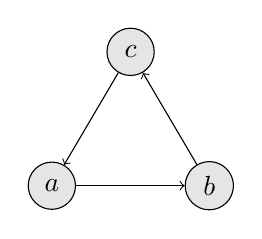
\begin{tikzpicture}[every node/.style={circle, draw=black, fill=gray!20, minimum size=0.6cm}]
        \node (a) at (0,0) {$a$};
        \node (b) at (2,0) {$b$};
        \node (c) at (1,1.7) {$c$};
        % Flechas seguras bajo babel «spanish»: la plantilla carga
        % \usetikzlibrary{babel}, sin la cual \draw[->] rompería.
        \draw[->] (a) -- (b);
        \draw[->] (b) -- (c);
        \draw[->] (c) -- (a);
    \end{tikzpicture}
    \caption{Ejemplo de figura en blanco y negro con TikZ: un
    digrafo con aristas dirigidas \texttt{->}.}
    \label{fig:grafo}
\end{figure}

La \cref{fig:grafo} muestra un digrafo de ejemplo, referenciado con
cleveref, que la llama «figura» por su \crefname en castellano; las
aristas dirigidas se escriben \texttt{->} con total normalidad porque
la plantilla neutraliza los caracteres abreviados de babel dentro de
TikZ.

\begin{definicion}
    Definición del segundo tema, con un párrafo algo más largo para
    que se aprecie de nuevo la sangría francesa en un entorno con
    varias líneas de texto seguidas.
\end{definicion}

\subsection{Primera subsección del tema}

Lorem ipsum dolor sit amet, consectetur adipiscing elit, sed do
eiusmod tempor incididunt ut labore et dolore magna aliqua.

\begin{teorema}
    Enunciado del teorema de la subsección.
\end{teorema}

\begin{demostracion}
    Demostración del teorema de la subsección.
\end{demostracion}

\subsubsection{Primera subsubsección}

Lorem ipsum dolor sit amet, consectetur adipiscing elit.

\begin{lstlisting}[style=python, caption={Ejemplo de fragmento de código en Python.}, label={lst:python}]
def hola(nombre):
    # Fragmento de código de ejemplo
    return "Hola, " + nombre
\end{lstlisting}

El \cref{lst:python} es un ejemplo de fragmento de código con su
\lstlistingname{} y su etiqueta referenciable; el algoritmo de
\cref{alg:euclides} muestra el entorno de pseudocódigo en castellano.

\begin{algorithm}[ht]
    \caption{Algoritmo de Euclides}\label{alg:euclides}
    \begin{algorithmic}[1]
        \Require $a, b \in \mathbb{N}$ con $a \geqslant b$
        \Ensure $\mathrm{mcd}(a, b)$
        \While{$b \neq 0$}
            \State $(a, b) \gets (b, a \bmod b)$
            % El \Comment usa ▷, que Fira Math no trae: lo aporta el
            % respaldo de Latin Modern Math fijado en el preámbulo.
            \Comment{resta con signo ignorado}
        \EndWhile
        \State \Return $a$
    \end{algorithmic}
\end{algorithm}

\subsection{Segunda subsección del tema}

\begin{table}[ht]
    \centering
    \begin{tabular}{|c|c|}
        \hline
        \textbf{Columna A} & \textbf{Columna B} \\ \hline
        1 & 2 \\ \hline
        3 & 4 \\ \hline
    \end{tabular}
    \caption{Ejemplo de tabla en blanco y negro.}
    \label{tab:ejemplo}
\end{table}

En \cref{tab:ejemplo} hay una tabla de ejemplo, y con \cref{tema:dos}
se referencia un tema completo; también se pueden cruzar referencias
con \cref{tema:uno} del primer tema.

\begin{problema}\label{prob:costes}
    Un problema con costes: comprar toneladas de un producto en
    varios proveedores, a $27\,\euro{}$ por tonelada en el mercado
    spot, minimizando el gasto total. Las comprobaciones de
    factibilidad de cada iteración se marcan con \ding{51} (sí)
    y \ding{55} (no), en blanco y negro, sin colores.
\end{problema}

\begin{resolucion}
    Resolución del problema de \cref{prob:costes}: fíjate en que la
    cabecera es «Resolución» (el argumento opcional la cambia) y en
    que, a diferencia de las demostraciones, NO termina con el
    cuadrado de QED. La matriz de incidencia del problema, de 11
    columnas, solo compila porque el preámbulo fija
    \texttt{MaxMatrixCols} a 20 (el límite de amsmath es 10):
    \[
    M =
    \begin{pmatrix}
        1 & 0 & 1 & 0 & 0 & 1 & 0 & 1 & 0 & 0 & 1 \\
        0 & 1 & 1 & 0 & 1 & 0 & 0 & 1 & 1 & 0 & 0 \\
        1 & 1 & 0 & 1 & 0 & 0 & 1 & 0 & 0 & 1 & 1 \\
    \end{pmatrix}
    \]
    La primera iteración es factible \ding{51} y la segunda no
    \ding{55}.
\end{resolucion}
